\typeout{Bewegingsherkenning met een smartphone}

\documentclass{article}
\usepackage[dutch]{babel}
\usepackage{ijcai11}
\usepackage{times}
\usepackage{tikz}
\usepackage{graphicx}
\usepackage{pgfplots}

\usepackage{subcaption}
%\usepackage{latexsym}  %optional

\title{Bewegingsherkenning met een smartphone}
\author{Arne De Brabandere\\
	arne.debrabandere@student.kuleuven.be
    \And
    Menno Keustermans\\
    menno.keustermans@student.kuleuven.be}
    
\tikzset{
    vertex/.style = {
        circle,
        fill            = black,
        outer sep = 2pt,
        inner sep = 1pt,
    }
}

\begin{document}

\maketitle

\begin{abstract}

Bewegingsherkenning is een belangrijke doelstelling van "context aware computing". Het gebruik van accelerometer gegevens geleverd door een smartphone zorgt ervoor dat een gegevensset snel geleverd kunnen worden. In het eerste deel van ons onderzoek hebben we gezocht naar een model om afzonderlijke activiteiten te herkennen. Het nauwkeurigste model werd gevonden met de classificatiemethode: RandomForest met 93\%. Vervolgens hebben we dit model gebruikt om een sequentie van verschillende bewegingen te evalueren. Het algoritme dat we hiervoor ontwikkeld hebben, knipt de sequentie in opeenvolgende tijdsvensters van x aantal seconden die ook met een bepaald percentage kunnen overlappingen. Uit experimenten bleek dat hiervoor een tijdsvenstergrootte van vier seconden met overlapping van 75\% het nauwkeurigst bleek te werken.

\end{abstract}

\section{Introductie}


\subsubsection{Geralateerd werk}
%TODO situering van het werk + bijdragen:
% - waarom bewegingen herkennen? (extra bronnen gebruiken
% - waarom met smartphones?
% - korte uitleg over onderzoek dat al gedaan is hierover voor afzonderlijke activiteiten (zie papers van literatuurstudie)
% - uitleg over eigen bijdrage: (1) van model om afzonderlijke activiteiten te herkennen naar algoritme om sequenties van activiteiten te herkennen (+ duidelijk zeggen wat we met afzondelijke activiteiten en sequenties bedoelen)



% bij 2 secties telkens "data collectie" + "data verwerking" + leermethodes + experimenten  +resultaten + conclusie

\section{Afzondelijke activiteiten}

Het eerste probleem is om van een gegeven reeks samples van de accelerometer en gyroscoop van een smartphone de activiteit van een persoon te bepalen. We veronderstellen hier dat telkens \'e\'en afzonderlijke activiteit gemeten wordt.

We willen tien verschillende activiteiten kunnen herkennen:
\begin{itemize}
\item wandelen,
\item lopen,
\item fietsen,
\item een trap opwandelen,
\item een trap afwandelen,
\item springen,
\item niets doen (zitten, liggen, staan),
\item een lift naar boven nemen, %TODO anders verwoorden? (want eigenlijk is het alleen de versnelling van een lift naar boven, en lift naar boven = versnelling naarboven + versnelling naar beneden)
\item een lift naar beneden nemen,
\item tanden poetsen.
\end{itemize}

In bovenstaande lijst hebben we tanden poetsen als moeilijke activiteit toegevoegd. De beweging lijkt sterk op niets doen en zal waarschijnlijk minder goed te herkennen zijn. Ook voor lift naar boven en trap opwandelen bestaan er gelijkaardige bewegingen, respectievelijk lift naar beneden en trap afwandelen.

Het proces om een afzonderlijke activiteiten te herkennen verloopt in drie stappen. Ten eerste moeten er gegevens verzameld worden. Als tweede stap worden er features berekend op de verzamelde gegevens. Deze zijn nodig om tenslotte modellen te leren met behulp van classificatiemethodes. Als criterium om de verschillende modellen te vergelijken, gebruiken we de accuraatheid als percentage van het aantal juiste geclassificeerde samples ten op zichte van het totaal aantal samples met behulp van cross-validatie.

%TODO ook motivatie (waarom classificatiemethodes)

\subsection{Gegevensverzameling}

Alle gegevens werd opgemeten door MotionTracker tool %TODO verwijzing met voetnoot: geschreven door ... 
. Dit is een Android-applicatie die de versnelling en rotatie (respectievelijk gemeten door de accelerometer en gyroscoop van de smartphone) aan 50 Hertz.  Als uitvoer geeft de applicatie een .log-bestand met de gemeten versnellingen (in de x-as, y-as en z-as met de z-as evenwijdig met de gravitatie) en rotaties (in quaternion notatie) met bijhorende timestamps.

Voor elke meting werd de applicatie gestart alvorens de smartphone in de broekzak gestopt werd en gestopt na het uithalen. Waardoor er bij het begin en einde van elke meting altijd enkele seconden niet-activiteit bevat. Om zo het fout labelen te vermijden, werd na elke meting een stuk van de start en het einde van het .log-bestand weggeknipt. Zodat elke meting exact \'e\'en activiteit bevat van vier \'a twintig seconden. 

We hebben voor elke activiteit 22 metingen verzameld, opgemeten door twee verschillende personen. Om voldoende variatie te hebben, gebeurden de metingen op verschillende dagen. Ook hebben we ervoor gezorgd dat we niet telkens dezelfde broek droegen, aangezien de gemeten versnelling kan vari\"eren in verschillende broekzakken. Na elke meting werd het uitgevoerde .log-bestand geknipt en gelabeld met de juiste activiteit.

%TODO figuur met verschillende activiteiten

\subsection{Gegevensverwerking: features berekenen}

Voor we classificatiemethodes kunnen gebruiken, moeten we eerst features berekenen. Dit zijn parameters die we uit de samples van de accelerometer en gyroscoop kunnen halen. Om de verschillende features te berekenen, maakten we gebruiken van MotionFingerPrint.jar tool %TODO verwijzing naar tool 


%TODO uitleggen waarom we features berekenen

MotionFingerPrint berekent in totaal 134 features verdeeld onder vier soorten:
\begin{itemize}
\item \textit{Statistische features:}
 dit zijn gemiddelde, standaardafwijking van zowel z- als xy-versnellingen en vermogen. En correlatie tussen z- en xy-versnelling.
 
\item \textit{Fourier-transformatie:} deze worden berekend in het frequentie domein van de metingen, zoals amplitudes volgens de verschillende assen.

\item \textit{Wavelet-transformatie:} %TODO

\item \textit{Hidden Markov models:} log-likelihood voor het model van elke activiteit
\end{itemize}

Het resultaat van de features berekening geeft een voor elke sample een set van parameters. Elke set vormt een instantie van de training set om een model te leren.

\subsubsection{Feature selectie}
%Waarom
Tussen de verschillende soorten features is er verschil in berekeningstijd en hoeveelheid informatie. Zo kunnen statistische features in het algemeen tegen een lagere kost berekend worden ten op zichte van fourier transformatie features. In sommige toepassingen kan het daarom interessant zijn om slechts een deel van het totaal aantal features te berekenen en juist degene die het meeste informatie bevatten.

%Voorgestelde Oplossing
Met behulp van feature selectie hebben we onderzocht hoeveel features van het totaal aantal features van elke soort nodig zijn om een redelijke accuraatheid te behalen. Om de features met het meeste informatie te vinden, maakten we gebruik van weka's: \emph{InfoGainAttributeEval} klasse. %TODO voetnoot naar weka informatie gain
 Deze klasse evalueert de waarde van elke features met behulp van information gain. Hierbij werd er steeds de entropie waarde berekend.

%Evaluatie
Vervolgens om de geselecteerde features te evalueren maakten we gebruik van dubbele cross-validatie. Bij de eerste cross-validatie (10-fold) werd de gegevensset verdeeld in een training- en testset. Daarna gebruikten we de gegeneerde training-set om de beste features te selecteren met het proces dat hierboven werd beschreven gebruik makend van de tweede cross-validatie (2-fold). Met de geselecteerde features werd een model opgesteld met behulp van de randomForest classificatiemethode. En dit model werd uiteindelijk getest om de testset die bij de eerste cross-validatie gemaakt werd.
	
%Resultaten
In figuur X worden de resulaten voor de verschillende soorten features getoond. We zien dat we met enkel de statistische features al een accuraatheid van 90\% behalen. Zelfs met de helft kan het model al vrij zeker de juiste activiteit voorspellen. We stellen vast dat van het grote aantal fourier tranformatie features slechts een tiental nodig zijn om een nauwkeurigheid van 80\% te bekomen. In het algemeen kunnen we kunnen concluderen dat wavelet transformatie functie minder goed werken (slechts 70\% accuraatheid). Tenslotte in de laatste grafiek merken we op dat de Hidden Markov Models enkel degelijk werken als alle features gebruikt worden.

%TODO figuur toevoegen

\begin{figure}[htb]
\centering

  \begin{subfigure}[b]{.49\linewidth}
    \centering
    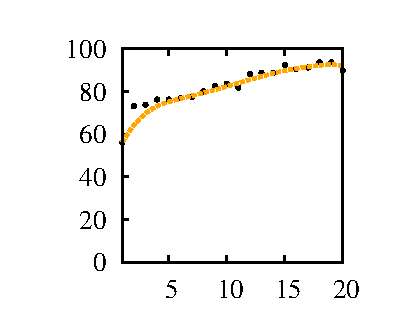
\includegraphics[width=0.99\textwidth]{figures/StatisticFeatures}
    \caption{Statistische features}\label{fig:1a}
  \end{subfigure}% 
  \begin{subfigure}[b]{.49\linewidth}
    \centering
    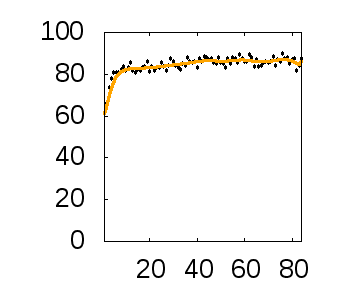
\includegraphics[width=.99\textwidth]{figures/FFTFeatures}
    \caption{FFT features}\label{fig:1b}
  \end{subfigure} \\
  \begin{subfigure}[b]{.49\linewidth}
    \centering
    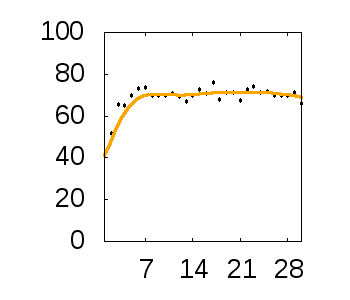
\includegraphics[width=.99\textwidth]{figures/DWTFeatures}
    \caption{Wavelet features}\label{fig:1c}
  \end{subfigure}
  \begin{subfigure}[b]{.49\linewidth}
    \centering
    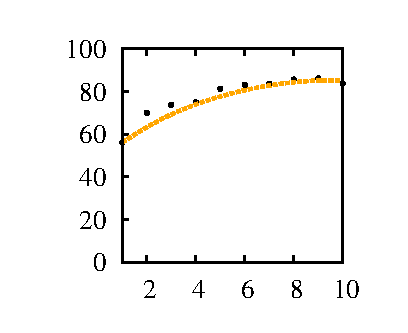
\includegraphics[width=.99\textwidth]{figures/HMMFeatures}
    \caption{HMM features}\label{fig:1e}
  \end{subfigure} \\
  

  \caption{Resultaten van het feature selectie experiment. Op de x-as wordt steeds het aantal features van de soort features geplot en op de y-as de accuraatheid in procenten.}\label{fig:1}
\end{figure}
Voor de rest van het onderzoek werd gebruik gemaakt van de volledige set features.



\subsection{Classificatiemethodes}

We gebruiken classificatiemethodes om een model te zoeken om afzonderlijke activiteiten te herkennen. We vergelijken enkele veel voorkomende methodes: beslissingsbomen, Random Forest, k-Nearest Neighbours, Naive Bayes en Support Vector Machines. De methodes leren telkens een model uit de instanties met de hierboven beschreven features voor de verschillende activiteiten. Hieronder wordt kort de werking van de vernoemde methodes beschreven:

\begin{itemize}
\item \textit{Beslissingsbomen} zijn bomen waarvan de interne knopen features voorstellen en de bladknopen \'e\'en (of meerdere) labels bevatten. Een tak in de boom stelt een test voor op de feature van de knoop waaruit de tak vertrekt. Om een nieuwe instantie te classificeren worden de juiste takken gevolgd tot in een bepaalde bladknoop. De instantie wordt dan geclassificeerd als het label in die bladknoop.
\item \textit{Random Forests} zijn combinaties van beslissingsbomen met een willekeurig deel van de trainingset en een willekeurig deel van de features. Bij de classificatie van een nieuwe instantie `stemt' elke boom op een label. De instantie krijgt vervolgens het label met de meeste stemmen.
\item \textit{k-Nearest Neighbours} classificeert nieuwe instanties door te zoeken naar de k dichtstbijzijnde instanties in de trainingset. Dit zijn de instanties waarvan de waarden voor de features het dichtst bij die van de te classificeren instantie ligt. Hieruit wordt het meest voorkomende label gekozen.
\item \textit{Naive Bayes} is een probabilistische classifier die gebruik maakt van voorwaardelijke kansen. De kans op een label $C$ met gegeven waarden voor de features $\mathbf{F}=(F_1, ..., F_n)$ wordt berekend als $P(C|\mathbf{F}) = { P(\mathbf{F}|C) P(C) \over P(\mathbf{F}) }$ waarin $P(\mathbf{F}|C)$, $P(C)$ en $P(\mathbf{F})$ uit de trainingset kunnen berekend worden. Bij het classificeren wordt het label met de grootste kans gekozen.
\item \textit{Support Vector Machines} beschouwt de features als een multidimensionele ruimte. De instanties zijn dan punten in de featureruimte. Bij het leren worden de instanties lineair van elkaar gescheiden door hypervlakken, zodat de instanties aan de ene kant van het vlak een ander label hebben dan die aan de andere kant. Wanneer de instanties niet lineair te scheiden zijn, worden ze getransformeerd met een \textit{kernel functie}. We gebruiken hier LibSVM, %TODO bron
waarbij binaire (\'e\'en-tegen-\'e\'en) classificatie gedaan wordt: elk hypervlak scheidt de instanties van 2 verschillende labels. Een nieuwe instantie wordt geclassificeerd door elke binaire classificatie als een stem voor een label te beschouwen. Het label met het grootste aantal stemmen wordt gekozen.
\end{itemize}

\subsection{Experimenten en resultaten}

We evalueren de methodes met 10-fold cross-validatie. Hierbij worden de instanties op 10 verschillende manieren opgesplitst zodat telkens 90\% van de instanties als trainingset wordt gebruikt om een model uit te leren. Op de overige 10\% wordt het model ge\"evalueerd. De accuraatheid van elke methode wordt dan berekend als het gemiddelde percentage van correct geclassificeerde instanties in de verschillende testsets.

In figuur \ref{methodes}
wordt de accuraatheid van de verschillende methodes vergeleken. We zien dat Random Forest de hoogste accuraatheid geeft voor onze metingen. Ook beslissingsbomen (J48) geeft een goede accuraatheid. De hogere accuraatheid van Random Forest ten opzichte van beslissingsbomen is te verklaren door het feit dat Random Forest minder kans op overfitting heeft.~\cite{breiman:randomforests}

\begin{figure}
\label{methodes}
\centering
\begin{tikzpicture}
\begin{axis}[
    ybar,
    xtick=data,
    ymin=0,
    xticklabels from table={Data/methodes.dat}{methode},
    xticklabel style={align=center},
    nodes near coords,
    ylabel={Accuraatheid (\%)}
]

\addplot table [
    x=xpos,
    y=accuraatheid
] {Data/methodes.dat};

\end{axis}
\end{tikzpicture}
\caption{Accuraatheid van classificatiemethodes}
\end{figure}

%TODO vermelden dat Random Forest het meest accurate model geeft in vergelijking met de modellen van de andere vier methodes

%TODO experimenten + resultaten: opsplitsen?

\section{Sequenties van activiteiten}

%TODO probleemstelling

\subsection{Datacollectie}

%TODO hoe hebben we de data verzameld

\subsection{Dataverwerking}

%TODO iets over het labelen + uitleg van tijdsvensters, overlappingen

\subsection{Algoritme}

%TODO algoritme uitleggen + hierbij ook uitleg over ruis-cutoff

\subsection{Experimenten en resultaten}

%TODO
% - hoe gebeurt de evaluatie?
% - accuraatheid plotten in functie van grootte van tijdsvensters en overlap + tijdsvensters vergelijken + iets over ruis cut-off
%   ==> hypothese (waarschijnlijk 4sec en 3/4 overlap, omwille van activiteit lift versnelt omhoog/omlaag)
% - bespreking van resultaten: komt dit overeen met de hypothese?

\section{Conclusie}

%TODO voor afzonderlijke activiteiten EN (?) voor sequenties

\section{Verder werk}

%TODO misschien wat er zou gebeuren als hetzelfde zou gedaan worden voor meer metingen? (bvb. wandelen, lopen, ... accurater)




%TODO bronvermelding!

%% The file named.bst is a bibliography style file for BibTeX 0.99c
% \bibliographystyle{named}
% \bibliography{paper}

\end{document}

